\documentclass[answers]{exam}
\usepackage{../../template}
\title{Assignment 3}
\author{Daniel Chua}
\begin{document}
\maketitle

% 3b
% 5
\begin{questions}

\question{Using the tables for $\langle \sigma v\rangle_{D^3He}$ in Dolan find the ideal ignition temperature for a D-3He plasma ($n_D = n_{He}$). Use the graph in Dolan for $\langle \sigma v\rangle_{pB}$ to estimate the ideal ignition temperature for proton-boron fusion with $n_B/n_p = 1/3$ (consider only bremsstrahlung radiation losses). Find the optimum p-B concentrations to maximize $P_f/P_{br}$.}

\begin{solution}
    % p = nkT, r = n n sigma v, T big -> sigma v big, but n small, prolly just try for many values
    % balance power of charged particles and power of bremsstrahlung, equal to 5e-37 sum_i n_en_iz_i^2 sqrt(T_e)
    % assume DD reactions are negligible, however, this is a bad assumption, since they aren't
    Bremsstrahlung losses are
    \begin{align*}
        P_{br} &= 5\times10^{-37} \sum_i n_en_iz_i^2 \sqrt{T_e} \\
               &= 5\times10^{-37} \sqrt{T_e} (n_en_D + 4n_en_{He}) \\
               &= 2.5\times10^{-36} \sqrt{T_e} n_en_D \\
               &= 2.5\times10^{-36} \sqrt{T_e} (n_D + 2n_{He}) n_D \\
               &= 7.5\times10^{-36} \sqrt{T_e} n_D^2
    \end{align*}
    where $T_e$ has units of keV. Power gain is
    \begin{align*}
        P_\alpha &= rE \\
          &= 14.6 \times 10^6 \times 1.6 \times 10^{-19} n_Dn_{He}\overline{\sigma v} \\
          &= 2.336 \times 10^{-12} n_Dn_{He}\overline{\sigma v}
    \end{align*}
    For ideal ignition, we want
    \begin{align*}
        P_\alpha &= P_{br} \\
        2.336 \times 10^{-12} n_D^2 \overline{\sigma v} &= 7.5 \times 10^{-36} \sqrt{T_e} n_D^2 \\
        \overline{\sigma v} &= 3.21 \times 10^{-24} \sqrt{T_e}
    \end{align*}
    We then try to find a $T_e$ that minimises the difference between the first and second term.
    \begin{center}
    \begin{tabular}{|c|c|}
        \hline
        Temperature & Difference \\
        \hline\hline
        1 & $-3.21\times10^{-24}$ \\
        \hline
        10 & $-9.53\times10^{-24}$ \\
        \hline
        20 & $-1.16 \times 10^{-23}$ \\
        \hline
        40 & $-1.20 \times 10^{-23}$ \\
        \hline
        80 & $-9.42 \times 10^{-24}$ \\
        \hline
        100 & $-2.11 \times 10^{-23}$ \\
        \hline
        150 & $-3.52 \times 10^{-24}$ \\
        \hline
        200 & $7.95 \times 10^{-25}$ \\
        \hline
    \end{tabular}
    \end{center}
    \bigskip
    The ideal temperature is 200 keV. For proton boron fusion,
    \begin{align*}
        P_{br} &= 5\times10^{-37} \sum_i n_en_iz_i^2 \sqrt{T_e} \\
               &= 5\times10^{-37} \sqrt{T_e} (25n_en_B + n_en_p) \\
               &= 5\times10^{-37} \sqrt{T_e} (28n_en_B) \\
               &= 5\times10^{-37} \sqrt{T_e} \left(112n_B^2\right) \\
               &= 5.6\times10^{-35} \sqrt{T_e} n_B^2
    \end{align*}
    and power is
    \begin{align*}
        P_f &= rE \\
          &= 8.68 \times 10^6 \times 1.6 \times 10^{-19} n_Bn_p\overline{\sigma v} \\
          &= 1.39 \times 10^{-12} 3n_B^2 \overline{\sigma v} \\
          &= 4.17 \times 10^{-12} n_B^2 \overline{\sigma v}
    \end{align*}
    Similarly, we want to minimise the difference between the left and right terms.
    \begin{align*}
        P_f &= P_{br} \\
        4.17 \times 10^{-12} \overline{\sigma v} &= 5.6 \times 10^{-35} \sqrt{T_e} n_B^2 \\
        \overline{\sigma v} &= 1.34 \times 10^{-23} \sqrt{T_e}
    \end{align*}
    At $T \approx 158.7 \unit{keV}$ (two-thirds between 100 and 200 on a log graph) the difference is $-6.47 \times 10^{-21} < 0$, but at $T = 200 \unit{keV}$, the difference is $4.13 \times 10^{-22} > 0$. Then 200 keV is approximately the ideal ignition temperature. \\
    To optimise the p-B concentration, let $k = \frac{n_B}{n_p}$. Then
    \begin{align*}
        \frac{P_f}{P_{br}} &= \frac{rE}{5\times10^{-37} \sum_i n_en_iz_i^2 \sqrt{T_e}} \\
                           &\propto \frac{n_Bn_p\overline{\sigma v}}{25n_en_B + n_en_p} \\
                           &\propto \frac{kn_p^2}{25k(k+1)n_p^2 + (k+1)n_p^2} \\
                           &\propto \frac{k}{25k^2 + 26k + 1}
    \end{align*}
    Differentiating and setting to 0,
    \begin{align*}
        \frac{25k^2 + 26k + 1 - k(50k + 26)}{\left(25k^2 + 26k + 1\right)^2} &= 0 \\
        -25k^2 + 1 &= 0 \\
        k &= \frac{1}{5}
    \end{align*}
    The ideal concentration is then
    $$\frac{n_B}{n_p} = \frac{1}{5}$$
\end{solution}

\question{Consider a D–T plasma with $n_T = 2/3n_D$ and a nitrogen contamination level of $n_N/n_e = 0.05$. Assume $T_e = 3/4T_i$ with $T_D = T_T = T_N = T_i$ and that $T_i$ is high enough that the nitrogen is full ionized and its line radiation can be neglected compared with its bremsstrahlung radiation.}

\begin{parts}
    
\part{Use the plasma quasi-neutrality relation to find the fuel dilution factor $(n_D/n_e)^2$ and $Z_{\text{eff}}$.}

\begin{solution}
    Assuming everything is fully ionized,
    $$n_e = n_D + n_T + 7n_N$$
    Substituting the two given relations,
    \begin{align*}
        n_e &= n_D + \frac{2}{3} n_D + 7 \times 0.05 n_e \\
        0.65n_e &= \frac{5}{3} n_D \\
        \left(\frac{n_D}{n_e}\right)^2 &= 0.1521
    \end{align*}
    We can use the formula to find
    \begin{align*}
        Z_{\text{eff}} &= \sum_i \frac{n_i}{n_e} Z_i^2 \\
                       &= \frac{n_D}{n_e} + \frac{n_T}{n_e} + 49 \times \frac{n_N}{n_e} \\
                       &= 0.39 + 0.26 + 49 \times 0.05 \\
                       &= 3.1
    \end{align*}
\end{solution}

\part{Find the ignition temperature assuming only bremsstrahlung loss. Which "hurts" more, the fuel dilution or the radiation due to impurity?}

\begin{solution}
    \begin{align*}
        P_\alpha &= P_{br} \\
        \frac{4}{5} P_f &= 5 \times 10^{-37} \sum_i n_en_i z_i^2 \sqrt{T_e} \\
        rE &= 6.25 \times 10^{-37}n_e \sqrt{T_e} (0.39n_e + 0.26n_e + 49 \times 0.05n_e) \\
        17.59 \times 10^6 \times 1.6 \times 10^{-19} n_Dn_T \overline{\sigma v} &= 6.25 \times 10^{-37}n_e^2 \sqrt{T_e} \times 3.1 \\
        \overline{\sigma v} &= 6.79 \times 10^{-24} \sqrt{T_e}
    \end{align*}
    Then using the approximation
    $$\overline{\sigma v} \approx 5.1 \times 10^{-22} (\ln T_i - 2.1)$$
    we get
    $$T = 8.49\unit{keV}$$
    Without impurities,
    $$Z_{eff} = \frac{n_D + n_T}{n_e} = 1$$
    This is less than a third of that with impurities. Since this is a factor in calculating $P_{br}$, radiation due to impurity is significant, which fuel dilution is insignificant, as seen in the small value of $\frac{n_N}{n_e}$.
\end{solution}

\part{Derive a simple version of the Lawson Criterion. Evaluate $n_D\tau$ for $T_i = 10 \unit{keV}$. Compare with the result if $T_e = T_i = 10 \unit{keV}$. Comment.}

\begin{solution}
    \begin{align*}
        P_{in} &= P_{out} \\
        \varepsilon P_f &= (1 - \varepsilon) \sum \frac{3}{2} \frac{nkT}{\tau} \\
        P_f &= \frac{3k}{\tau} \left(n_eT_e + n_DT_D + n_TT_T + n_NT_N\right) \\
        17.59 \times 10^6 \times 1.6 \times 10^{-19} n_Dn_T \overline{\sigma v} &= \frac{3kT_i}{\tau} \left(\frac{3}{4} n_e + 0.39n_e + 0.26n_e + 0.05n_e\right) \\
        7.32 \times 10^{-13} n_D \overline{\sigma v} &= \frac{3kT_i}{\tau} \times 1.45 \\
        n_D\tau &= 8.21 \times 10^{-11} \frac{T_i}{\sigma v}
    \end{align*}
    At 10 keV, $n_D\tau = 8.21 \times 10^{-10} \times \frac{10,000 \times 11606}{0.582 \times 10^{-24}} = 1.64 \times 10^{22}$. If we assume $T_e = T_i$, the equation would become
    $$n_D\tau = 9.62 \times 10^{-11} \frac{T_i}{\sigma v} = 1.92 \times 10^{22}$$
    This shows that having a slightly lower $T_e$ can loosen the Lawson Criterion.
\end{solution}

\part{If $n_e = 2 \times 10^{20} \unit{m^{-3}}$ and $\beta = 6\%$ find the magnetic field required to maintain the plasma at ignition conditions. Does the impurity “help” or “hurt” in this case?}

\begin{solution}
    \begin{align*}
        \beta &= \frac{2\mu_0}{B^2} \sum nkT \\
        0.06 &= \frac{2\mu_0}{B^2} n_ekT_i (0.75 + 0.39 + 0.26 + 0.05) \\
        B^2 &= 1.946T_i \\
        B &= 4.07\unit{T}
    \end{align*}
    The impurity hurts in this case, because it causes $\sum nkT$ to increase, so $B$ also needs to grow to compensate.
\end{solution}

\part{The energy confinement time $\tau_E$ is defined to be the ratio of the energy content of the plasma to the energy loss rate. Allowing for bremsstrahlung loss only, what is the confinement time for the present plasma at $n_e = 2 \times 10^{20} \unit{m^{-3}}$ and $T_i = 10 \unit{keV}$?}

\begin{solution}
    \begin{align*}
        P_{br} &= 5 \times 10^{-37} \sum_i n_in_ez_i^2 \sqrt{T_e} \\
               &= 5 \times 10^{-37} n_e^2 \sqrt{T_e} (0.39 + 0.26 + 49 \times 0.05) \\
               &= 9.80 \times 10^{-16}n_e
    \end{align*}
    Then
    \begin{align*}
        \tau_E &= \frac{\frac{3}{2} \sum nkT}{P_{br}} \\
               &= \frac{2.175n_ekT_i}{9.80 \times 10^{-16}n_e} \\
               &= \frac{2.175kT_i}{9.80 \times 10^{-16}} \\
               &= 3.56
    \end{align*}
\end{solution}
\end{parts}

\question{}

\begin{parts}

\part{Show that the Lawson Criterion for D–T fusion is the given expression where $\tau$ is the energy replacement time for all losses and the energy conversion efficiency is $\varepsilon = 1/3$. Plot $n_i\tau$ vs. $T_i$ for various values of $T_i/T_e$. Comment}

\begin{solution}
    We assume $n_D = n_T = \frac{1}{2}n_i = \frac{1}{2}n_e$.
    \begin{align*}
        P_{in} &= P_{out} \\
        \varepsilon P_f &= (1 - \varepsilon) \sum \frac{3}{2} \frac{nkT}{\tau} \\
        P_f &= \frac{3k}{\tau} \left(n_eT_e + n_DT_D + n_TT_T\right) \\
        E_{DT} n_Dn_T \overline{\sigma v} &= \frac{3k}{\tau} \left(n_eT_e + n_iT_i\right) \\
        \frac{1}{4} E_{DT} n_i^2 \overline{\sigma v} &= \frac{3k}{\tau} n_i (T_e + T_i) \\
        n_i\tau &= \frac{12k(T_e+T_i)}{E_{DT}\overline{\sigma v}} \\
                &= \frac{12kT_e(1 + T_i/T_e)}{E_{DT}\overline{\sigma v}}
    \end{align*}
    \begin{center}
        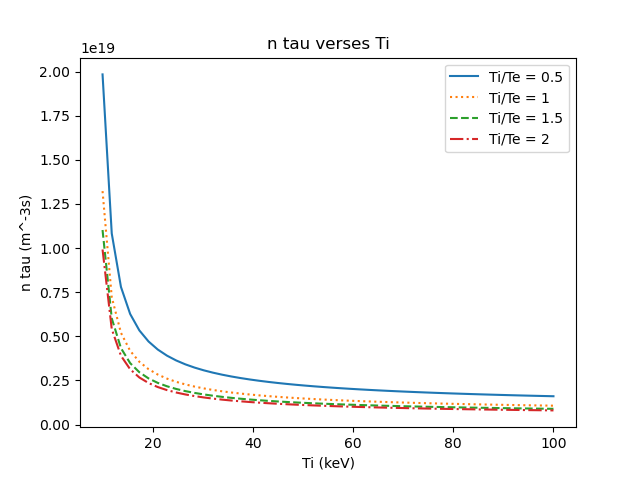
\includegraphics{q3a.png}
    \end{center}
    This implies that Lawson's Criterion is loosened as the ratio $T_i/T_e$ increases.
\end{solution}

\part{Assume $T_e = T_i$ and use the definition for the energy gain factor: $Q \equiv P_f/P_{in}$. If $n_i\tau = 1.5 \times 10^{20} \unit{m^{-3}.s}$, at what value of $T$ will $Q = 4$? $Q = 6$? Comment.}

\begin{solution}
    Recall
    $$\tau = \frac{3n_ikT}{P_{in}}$$
    Then
    \begin{align*}
        Q &= \frac{P_f}{P_{in}} \\
          &= E_{DT} n_Dn_T\overline{\sigma v} \times \frac{\tau}{3n_ikT} \\
          &= 17.59 \times 10^6 \times 1.6 \times 10^{-19} \frac{n_i^2}{4} \overline{\sigma v} \times \frac{\tau}{3n_ikT} \\
          &= 2.195 \times 10^{23} \times \frac{\overline{\sigma v}}{T} \\
          &= 2.195 \times 10^{23} \times 5.1 \times 10^{-22} \frac{\ln T_i - 2.1}{T} \\
          &= 112 \frac{\ln T_i - 2.1}{T}
    \end{align*}
    Something went wrong, because there are no solutions for both $Q=4$ and $Q=6$...
\end{solution}

\part{Show that the Lawson criterion for DT fusion can also be written as follows.}

\begin{solution}
    \begin{align*}
        P_{in} + P_\alpha &= P_{loss} \\
        \frac{\varepsilon}{1-\varepsilon}P_f + E_\alpha \frac{n_i^2}{4} \overline{\sigma v} &= \frac{\sum \frac{3}{2} nkT}{\tau} + P_{br} + K_{cy}P_{cy} \\
        \frac{1}{2} E_{DT} \frac{n_i^2}{4} \overline{\sigma v} + \frac{1}{4} E_\alpha n_i^2 \overline{\sigma v} &= \frac{3n_ikT}{\tau} + C_1n_i^2T^{1/2} + C_2n_i^2T^2 \\
        \frac{1}{8} E_{DT} \overline{\sigma v} + \frac{1}{4} E_\alpha \overline{\sigma v} - C_1T^{1/2} + C_2T^2 &= \frac{3kT}{\tau n_i} \\
        n_i\tau &= \frac{3kT}{\frac{1}{8} E_{DT} \overline{\sigma v} + \frac{1}{4} E_\alpha \overline{\sigma v} - C_1T^{1/2} + C_2T^2}
    \end{align*}
\end{solution}

\part{For $\beta = 5\%$ and $n_{imp} = 0$, plot $n_i\tau$ vs. $T$ and compare with part (a). Assume $K_{cy} = 1, 0.01$. Comment.}


\begin{solution}
    From Bremsstrahlung, the constant term $C_1$ is
    $$C_1 = 5 \times 10^{-37}$$
    If $n_{imp} = 0$, we have $n_e = n_i$. Simplifying for $P_{cy}$, we obtain
    $$C_2 = 2.5 \times 10^{-38} \times 2 \div 5\% = 1 \times 10^{-36}$$
    The other terms in the denominator are
    \begin{align*}
        \frac{1}{8}\overline{\sigma v}E_{DT} + \frac{1}{4} \overline{\sigma v}E_\alpha &= \overline{\sigma v} (\frac{1}{8} E_{DT} + \frac{1}{5} E_{DT}) \\
                                                                                       &= 5.11 \times 10^{-22} (\ln T_i - 2.1) \times \frac{13}{40} \times 17.59 \times 10^6 \times 1.6 \times 10^{-19} \\
                                                                                       &= 4.67 \times 10^{-34} (\ln T_i - 2.1)
    \end{align*}
    We can then plot the function.
    \begin{center}
    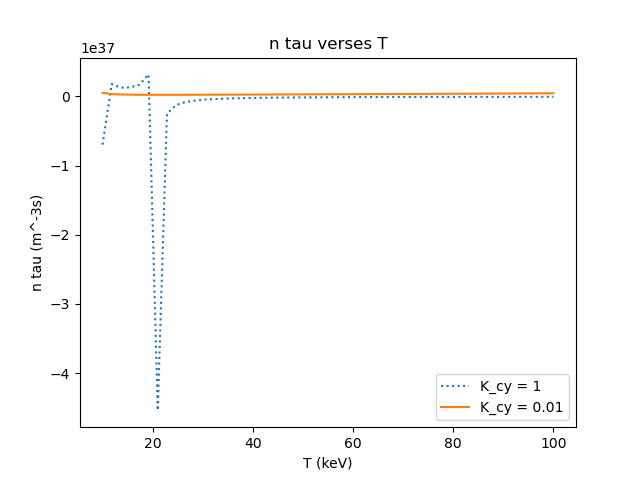
\includegraphics{q3d.png}
    \end{center}
    Comparing with 3(a), this implies that cyclotron radiation has a great effect on Lawson's Criterion (measured in orders of magnitude). Hence it should be minimised whenever possible. When $K_cy$ is reduced to 0.1, $n\tau$ vanishes on the graph, which makes sense, since the Criterion derived assuming only bremsstrahlung losses is around 10 orders of magnitudes smaller.
\end{solution}
\end{parts}

\question{Find $P_{cy}$ for D-D or D-T fusion.}

\begin{solution}
    First we find $\beta$. For charge to be balanced,
    $$n_e = n_D + n_T + n_{imp}Z_{imp}$$
    Then
    \begin{align*}
        \beta &= \frac{2\mu_0}{B^2} \sum nkT \\
              &= \frac{2\mu_0}{B^2} kT(n_D + n_T + n_{imp} + n_e) \\
              &= \frac{2\mu_0}{B^2} kT(n_D + n_T + n_{imp} + Z_{imp}n_{imp} - Z_{imp}n_{imp} + n_e) \\
              &= \frac{2\mu_0}{B^2} kT(2n_e + (1 - Z_{imp})n_{imp}) \\
              &= \frac{2\mu_0}{B^2} n_ekT(2 + f_{imp}(1 - Z_{imp}))
    \end{align*}
    Then substituting,
    \begin{align*}
        P_{cy} &= \frac{e^4B^2n_ekT}{3\pi\varepsilon_0m_e^3c^3} \\
               &= \frac{2\mu_0e^4n_e^2(kT)^2[2+f_{imp}(1-Z_{imp})]}{3\pi\varepsilon_0m_e^3c^3\beta}
    \end{align*}
    Evaluating the expression using all the constants, we have
    $$\frac{2\mu_0e^4k^2}{3\pi\varepsilon_0m_e^3c^3} = 1.84 \times 10^{-52}$$
    When using keV as the units for temperature, this is multiplied by a factor of $(11606 \times 1000)^2$ which yields the factor $2.5 \times 10^{-38}$. Then
    $$P_{cy} = 2.5 \times 10^{-38} n_e^2T^2[2 + f_{imp}(1 - Z_{imp})]/\beta$$
\end{solution}

\question{Confirm the value of the maximum permitted silicon content at T = 10 keV in Fig. 4B2 (p 79) of Dolan.}

\begin{solution}
    From Fig 4B2, the maximum permitted silicon content is $1.5 \times 10^{-2} = 1.5\%$. We attempt to verify this. \\
    Letting $x = \frac{n_{si}}{n_e}$, we can express
    \begin{align*}
        n_e &= n_i + 14n_{si} \\
            &= n_i + 14xn_e \\
            &= \frac{n_i}{1-14x}
    \end{align*}
    The radiation power of silicon is around $10^{-33}$ according to Fig 3F4. Then
    \begin{align*}
        P_{si,rad} &= 1.848 \times 10^{-33} n_en_{si} \\
                   &= 1.848 \times 10^{-33} n_e^2x \\
                   &= \frac{1.848 \times 10^{-33}xn_i^2}{(1-14x)^2}
    \end{align*}
    Now power of charged particles is
    \begin{align*}
        P_\alpha &= \frac{4}{5} P_f \\
                 &= \frac{4}{5} E_{DT} n_Dn_T \overline{\sigma v} \\
                 &= \frac{4}{5} \times 17.59 \times 10^6 \times 1.6 \times 10^{-19} \frac{n_i^2}{4} \times 0.582 \times 10^{-24} \\
                 &= 3.28 \times 10^{-37} n_i^2
    \end{align*}
       Hydrogenic bremsstrahlung radiation is
    \begin{align*}
        P_{br} &= 5 \times 10^{-37} \sum_i n_en_iz_i^2 \sqrt{T_e} \\
               &= 5 \times 10^{-37} n_en_i \sqrt{10} \\
               &= 1.58 \times 10^{-36} \frac{n_i^2}{1-14x}
    \end{align*}
    Cyclotron radiation is
    \begin{align*}
        P_{cy} &= 2.5 \times 10^{-38} n_e^2 T^2 [2 + f_{imp}(1 - Z_{imp})]/\beta \\
               &= 2.5 \times 10^{-38} \frac{n_i^2}{(1-14x)^2} \times 10^2 [2 + x(1 - 14)] \div 0.06 \\
               &= 4.17 \times 10^{-35} \times \frac{(2 - 13x)n_i^2}{(1 - 14x)^2}
    \end{align*}
    We use the ignition condition
    \begin{align*}
        P_\alpha &= P_{si, rad} + P_{br}^H + K_{cy}P_{cy} \\
        3.28 \times 10^{-37}n_i^2 &= \frac{10^{-33}xn_i^2}{(1-14x)^2} + 1.58 \times 10^{-36} \frac{n_i^2}{1-14x} + 4.17 \times 10^{-35} K_{cy} \times \frac{(2-13x)n_i^2}{(1-14x)^2} \\
        ax^2 + bx + c &= 0
    \end{align*}
    where
    \begin{align*}
        a &= 6.42 \times 10^{-35} \\
        b &= -9.99 \times 10^{-33} + 5.42 \times 10^{-34}K_{cy} \\
        c &= -1.24 \times 10^{-36} - 8.33 \times 10^{-35}K_{cy}
    \end{align*}
    For $K_{cy} = 1, x = 20.2$ or -0.0652. For $K_{cy} = 0.01, x = 28.5$ or $-1.14 \times 10^{-3}$. I was unable to get a correct value (between 0 and 1).

    % silicon isn't necessarily fully ionized; ignition condition Palpha = PSirad + Pbr^H + KcyPcy
    % H for hydrogen, bremsstrahlung included in PSirad
    % solve for x = nsi/ne
    % quadratic
\end{solution}

\end{questions}

\end{document}
